\documentclass[a4paper, 12pt]{article}
\usepackage[utf8]{inputenc}
\usepackage[brazil]{babel}
\usepackage{amsmath}

\usepackage{graphicx}
\usepackage{color}
\usepackage{xcolor}

% Macros for proof-reading
\usepackage[normalem]{ulem} % for \sout
%\newcommand{\ra}{$\rightarrow$}
\newcommand{\ugh}[1]{\textcolor{red}{\uwave{#1}}} % please rephrase
\newcommand{\ins}[1]{\textcolor{blue}{\uline{#1}}} % please insert
\newcommand{\del}[1]{\textcolor{red}{\sout{#1}}} % please delete
\newcommand{\chg}[2]{\textcolor{red}{\sout{#1}}{\ra}\textcolor{blue}{\uline{#2}}} % please change

% Put edit comments in a really ugly standout display
\usepackage{ifthen}
\usepackage{amssymb}
\newboolean{showcomments}
\setboolean{showcomments}{true} % toggle to show or hide comments
\ifthenelse{\boolean{showcomments}}
  {\newcommand{\nb}[2]{
    \fcolorbox{gray}{yellow}{\bfseries\sffamily\scriptsize#1}
    {\sf\small$\blacktriangleright$\textit{#2}$\blacktriangleleft$}
   }
   \newcommand{\version}{\emph{\scriptsize$-$working$-$}}
  }
  {\newcommand{\nb}[2]{}
   \newcommand{\version}{}
  }

% General comment
\newcommand\info[1]{\nb{Info}{#1}}

% Single author comment
\newcommand\Leo[1]{\nb{Leo}{#1}}
\newcommand\Gui[1]{\nb{Gui}{#1}}
\newcommand\Davi[1]{\nb{Davi}{#1}}
\newcommand\Saulo[1]{\nb{Saulo}{#1}}
\newcommand\Ricardo[1]{\nb{Ricardo}{#1}}

\newcommand\pca{Análise de Componentes Principais}

\title{Comparação quantitativa da atuação parlamentar de partidos políticos utilizando a \pca}
\author{}
\date{}

\begin{document}
 
\maketitle 
 
\section*{Resumo}

Neste artigo propomos um método de comparação quantitativa entre as atuações de partidos políticos no poder legislativo.
Este método utiliza como entrada dados de votações dos parlamentares em plenário, processa estes dados com o algoritmo \pca\ (PCA), e apresenta como resultado um gráfico bidimensional em que pontos representam partidos, e no qual a distância entre esses pontos reflete a semelhança entre os votos realizados pelos parlamentares. 

\section{Introdução}
\label{sec:intro}

%Contexto
%Motivação / problema 
%questão
%solução, avaliação

O Brasil é uma jovem democracia com um sistema político-partidário bastante fragmentado.
Atualmente existem no Brasil X partidos políticos, sendo que pelo menos Y deles podem ser considerados pequenos partidos, pois não possuem qualquer representatividade no congresso nacional.
Este quadro torna muito difícil para que o eleitor compreenda as diferenças práticas e ideológicas entre os partidos políticos. Desta forma, tornam-se valiosos os procedimentos que permitam estabelecer comparações entre os partidos, em particular as comparações objetivas, por não dependerem de julgamento subjetivo dos analistas. 

Dentre os agentes políticos de interesse que atuem em nome de partidos políticos, os parlamentares apresentam uma particularidade que os tornam mais fáceis de serem analisados com uma abordagem quantitativa. Dois ou mais parlamentares podem ser objetivamente comparados analisando-se suas preferências em votações de proposições legislativas. Dois parlamentares são ``semelhantes'', ou ``próximos'', se tendem a votar igual na maioria das vezes. Dois executivos diferentes não podem ser comparados da mesma forma, pois dois executivos diferentes não resolvem exatamente o mesmo problema nas mesmas condições. Discursos ideológicos e programáticos podem ser comparados, mas dificilmente de forma quantitativa. 

A comparação entre dois parlamentares pode ser feita de forma bastante simples, como por exemplo medindo a porcentagem de acordo entre eles sobre um conjunto de votações. No entanto, comparar três ou mais parlamentares concomitantemente e dispô-los em algum tipo de escala não é trivial. Da mesma forma, modelar comparações entre partidos com base nos valores das votações também requer algum procedimento mais sofisticado.

Neste estudo utilizaremos a \pca\ (PCA) como ferramenta matemática para realizarmos a comparação de um dado conjunto de votações, a fim de estabelecermos semelhanças quantitativas entre os partidos políticos que atuaram neste conjunto de votações.

Nossas principais contribuições são:

\begin{itemize}
 \item uma modelagem matemática de votações parlamentares que fornece a entrada necessária ao algoritmo PCA;
 \item evidências de que é possível utilizar o PCA para comparar quantitativamente a atuação legislativa de partidos políticos.
\end{itemize}


Este artigo se organiza da seguinte forma: na Seção~\ref{sec:relacionados} apresentaremos outros métodos quantitativos utilizados na Ciências Políticas para comparação de votações parlamentares; na Seção~\ref{sec:pca} forneceremos uma breve descrição sobre o funcionamento da PCA em termos de entrada requerida e saída gerada, enquanto que na Seção~\ref{sec:metodo} descreveremos nossa modelagem matemática para gerar um conjunto de vetores a partir de dados de votações, de forma que esses vetores sejam entrada da PCA; na Secão~\ref{sec:resultado} descreveremos os resultados obtidos com a aplicação da técnica proposta em dados reais de votações parlamentares; por fim, na Seção~\ref{sec:conclusoes} apresentamos nossas conclusões.  

\section{Trabalhos relacionados}
\label{sec:relacionados}

Nominate

Problemas do nominate

% hipótese sobre o nominate: mais adequado para a política dos EUA
% então talvez não apropriado para analisar distâncias entre partidos (mas somente entre parlamentares)
% interessado em direita/esquerda, mas sem mt sentido para governismo/oposição


\section{A Análise de Componentes Principais}
\label{sec:pca}

A \pca\ (PCA) é o método estatístico mais popular para redução dimensional de grandes conjuntos de dados~\cite{DataMining2003}. A PCA realiza uma \emph{transformação linear} que recebe como entrada um conjunto de $N$ vetores\footnote{Um vetor é um conjunto ordenado de valores, em que casa posição é chamada de dimensão. Um exemplo de um vetor de 3 dimensões é $v = [10, 15, 12]$.} de dimensão $M$ e produz um outro conjunto de $N$ vetores de dimensão $M$, de tal forma que a maior parte da informação nos vetores de saída fica acumulada nas primeiras dimensões. \emph{Informação} aqui se refere às diferenças entre os vetores de um dado conjunto. Mais precisamente, a primeira dimensão da saída da PCA possuirá a maior variância entre seus elementos, enquanto que a segunda dimensão possuirá a segunda maior variância, e assim por diante. Esta propriedade nos permite reduzir a dimensão de um conjunto de dados com o mínimo de perda de informação possível.

Um exemplo didático é apresentado no livro ``Data Mining, Concepts, Models, Methods, and Algorithms'' \cite{DataMining2003}, em que um conjunto de dados com duas dimensões (pontos em um gráfico bidimensional) é reduzido para um conjunto de dados com apenas uma dimensão (pontos em uma reta). Na figura podemos observar como o eixo que determina a primeira dimensão do resultado da PCA garante a máxima variância  entre os dados. Qualquer outro eixo escolhido deixaria as projeções dos pontos do gráfico sobre o eixo mais próximas entre si do que podemos ver no eixo adotado na figura.

\begin{figure}
\center
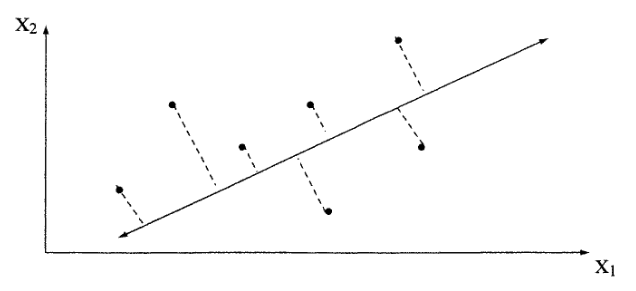
\includegraphics[scale=0.5]{img/pca}
\label{img:pca}
\caption{Exemplo de PCA aplicado na redução de 2 dimensões para 1 dimensão. Retirado de ``Data Mining, Concepts, Models, Methods, and Algorithms'' \cite{DataMining2003}}.
\end{figure}

Mostrar outros contextos em que o PCA é usado

\section{Método proposto}
\label{sec:metodo}

Conforme explicado na Seção~\ref{sec:pca}, a utilização da PCA requer como entrada um conjunto de vetores. Para que possamos utilizar a PCA para comparar partidos políticos objetivamente com base nos votos dados por parlamentares, precisamos então de uma modelagem matemática que gere um conjunto de vetores representativos de um dado conjunto de votações.

Nesta seção apresentaremos nossa proposta para a criação de \emph{vetores de votações} que sirvam de entrada para a PCA. Um vetor de votação modela as preferências de um partido político em um conjunto de votações. Dessa forma, aplicaremos a PCA com o objetivo de reduzir a dimensionalidade dos vetores de votação, tendo como saída de nosso algoritmo um conjunto de vetores de duas dimensões que podem ser representados como pontos em um gráfico bidimensional. Neste gráfico bidimensional gerado, cada ponto representará um partido, e quanto mais próximos um grupo de partidos estiverem no gráfico, mais semelhantemente terão esses partidos votado nas votações analisadas.

No caso mais simples, em que o partido possui apenas um parlamentar em uma dada casa legislativa, a i-ésima posição do vetor de votações é preenchido com um valor numérico correspondente ao valor do voto desse parlamentar na i-ésima votação do conjunto analisado. Esse valor numérico, correspondente ao voto de um parlamentar $d$ em uma votação $v$, é definido pela \emph{função opção}, $op(d,v)$, que é definida como se segue:

\[
   op(d,v) = \left\{ 
     \begin{array}{l l}
        1 & \text{, se parlamentar votou \emph{sim}} \\
       -1 & \text{, se parlamentar votou \emph{não}} \\
        0 & \text{, em algum outro caso} 
     \end{array} \right.
\]

Os ``outros casos'' além do sim e do não podem consistir na abstenção, ausência, ou mesmo obstrução. Todos esses casos representam uma impossibilidade em verificar a opinião do votante sobre a votação.

\Leo{TODO: enumerar suposições/premissas}

Formularemos agora a definição de um vetor de votações pertencente a um partido. Seja:

\begin{itemize}
 \item $C$ a casa legislativa sob análise;
 \item $p$ um partido político com representatividade em $C$;
 \item $D_p$ o conjunto dos parlamentares do partido $p$ em~$C$;
 \item $V = \{v_1, v_2, ..., v_n\}$ um conjunto de votações ocorridas em $C$.
\end{itemize}

Então o vetor de votações do partido $p$, representado por $vv_p$, será dado por:

\[
 vv_p[i] = \frac{ \sum_{d \in D_p}{op(d,v_i)} }{ |D_p| } \
\]

A fórmula acima expressa que a i-ésima posição do vetor de votações do partido $p$ possui como valor a média aritmética dos valores da função opção para todos os parlamentares do partido $p$ na votação $v_i$.

Exemplificando, assumamos o seguinte cenário: todos os parlamentares de $p$ votaram \emph{sim} na votação $v_1$; todos os parlamentares de $p$ votaram \emph{não} na votação $v_2$; todos os parlamentares de $p$ faltaram à votação $v_3$; e por fim, metade dos parlamentares de $p$ votaram \emph{sim} na votação $v_4$, mas a outra metade votou \emph{não} nessa mesma votação $v_4$. Nesta situação o vetor de votações do partido $p$ pode ser representado por $vv_p = [ 1, -1, 0, 0 ]$. 

O exemplo anterior evidencia como a abstenção e a ausência apresentam as mesmas consequências em nossa modelagem. Essa mesma consequência pode ser semanticamente interpretada como uma ``falta de opinião formada do partido sobre o assunto''. Claro que na realidade os parlamentares podem efetuar manobras, como baixar o quórum para impedir a votação, situação na qual se torna difícil entender se o partido seria a favor do \emph{sim} ou do \emph{não}. Desta forma, assumimos essa simplificação para permitir que nosso método se mantenha puramente quantitativo, sem que seja necessário a inserção do julgamento de analistas.

Os vetores de votação gerados pelo procedimento explicado serão fornecidos como entrada da \pca.
Ao aplicar a PCA sobre esses vetores de votações teremos como saída um novo conjunto de vetores de votação, mas com suas diferenças acumuladas nas primeiras dimensões. Dessa forma, o resultado final é apresentado em um gráfico de duas dimensões, cujos pontos possuem coordenadas correspondentes às duas primeiras dimensões dos vetores gerados pela PCA.

Na próxima seção descreveremos os resultados obtidos aplicando-se a PCA com a modelagem aqui apresentada a dados reais de votações parlamentares.

\section{Resultados}
\label{sec:resultado}

Mostrar gráficos e gerados 

% análise de variância por dimensão: mostra o quão bom está o 2D

\section{Conclusões}
\label{sec:conclusoes}

% resultados
% coisas pra melhorar / investigar
% ex: modelagem de partidos q não votam em alguma votação; suplentes; troca de parlamentares análise de sensibilidade

% trabalhos futuros: comparação rigorosa com o nominate

\bibliography{refs}
\bibliographystyle{plain}
 
\end{document}
